\documentclass{standalone}
\usepackage{tikz}
\usepackage{ctex,siunitx}
\usepackage{tkz-euclide}
\usepackage{amsmath}
\usetikzlibrary{patterns, calc}
\usetikzlibrary {decorations.pathmorphing, decorations.pathreplacing, decorations.shapes,}
\begin{document}
\small
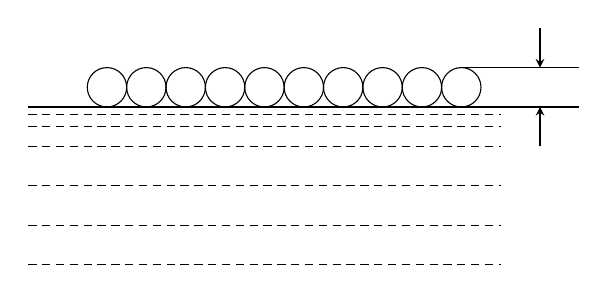
\begin{tikzpicture}[>=stealth]
  \draw (0,0)--(6,0);
  \foreach \x in {-.1, -.25, -.5, -1, -1.5, -2}
  { 
     \draw [densely dashed](0,\x)--(6,\x);
  }
  \foreach \y in {1,2,...,10}
  {
     \draw (\y/2+.5,.25) circle [radius=.25];
  }
  \draw [thin] (5.5,0)--(7,0);
  \draw [thin] (5.5,.5)--(7,.5);
  \draw [->,thin](6.5,1.0)--(6.5,.5);
  \draw [->,thin](6.5,-0.5)--(6.5,0);
  \end{tikzpicture}
\end{document}